% Preview of the thesis figures at their final size (A4, 11pt, text width 15.9 cm = 6.27 in).
% Compile in analysis/summary/figures/: pdflatex _preview.tex
\documentclass[11pt,a4paper]{report}
\usepackage[a4paper,textwidth=15.9cm,vmargin=2.5cm]{geometry}
\usepackage{graphicx,amsmath,lmodern}
\usepackage[T1]{fontenc}
\begin{document}

\begin{figure}[p]
  \centering
  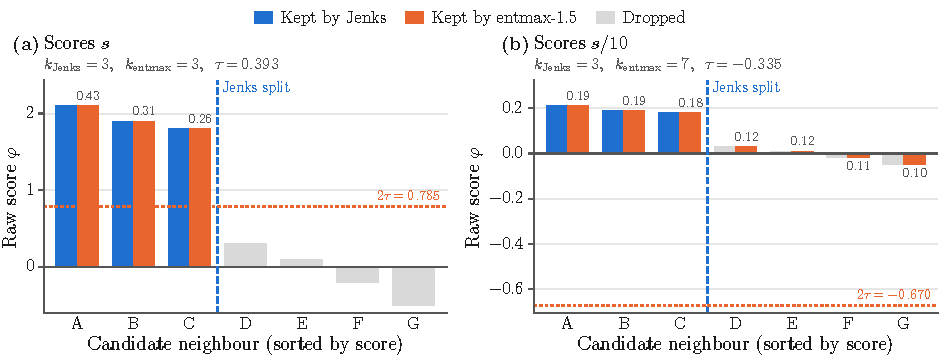
\includegraphics[width=\textwidth]{selection_example.pdf}
  \caption[selection example]{Neighbour selection of the two adaptive rules on one node with seven candidate neighbours A--G, raw scores $s = (2.1, 1.9, 1.8, 0.3, 0.1, -0.2, -0.5)$ in (a) and the same scores divided by 10 in (b). For each candidate, the left bar is coloured if the Jenks rule keeps it and the right bar if entmax-1.5 keeps it (grey: dropped). Jenks splits the sorted scores into two natural-breaks classes (dashed line) and keeps the upper class; entmax-1.5 assigns $p_j = [s_j/2 - \tau]_+^2$ with $\sum_j p_j = 1$ and keeps every candidate with $p_j > 0$, i.e.\ $s_j > 2\tau$ (dotted line); the numbers above the bars are $p_j$. The Jenks split depends only on the shape of the score row, so it keeps three neighbours in both panels, whereas entmax-1.5 keeps three in (a) and all seven once the scores are flatter (b). The kept sets were computed by the model's own adjacency module on these scores (no training involved).
}
  \label{fig:selection_example}
\end{figure}

\begin{figure}[p]
  \centering
  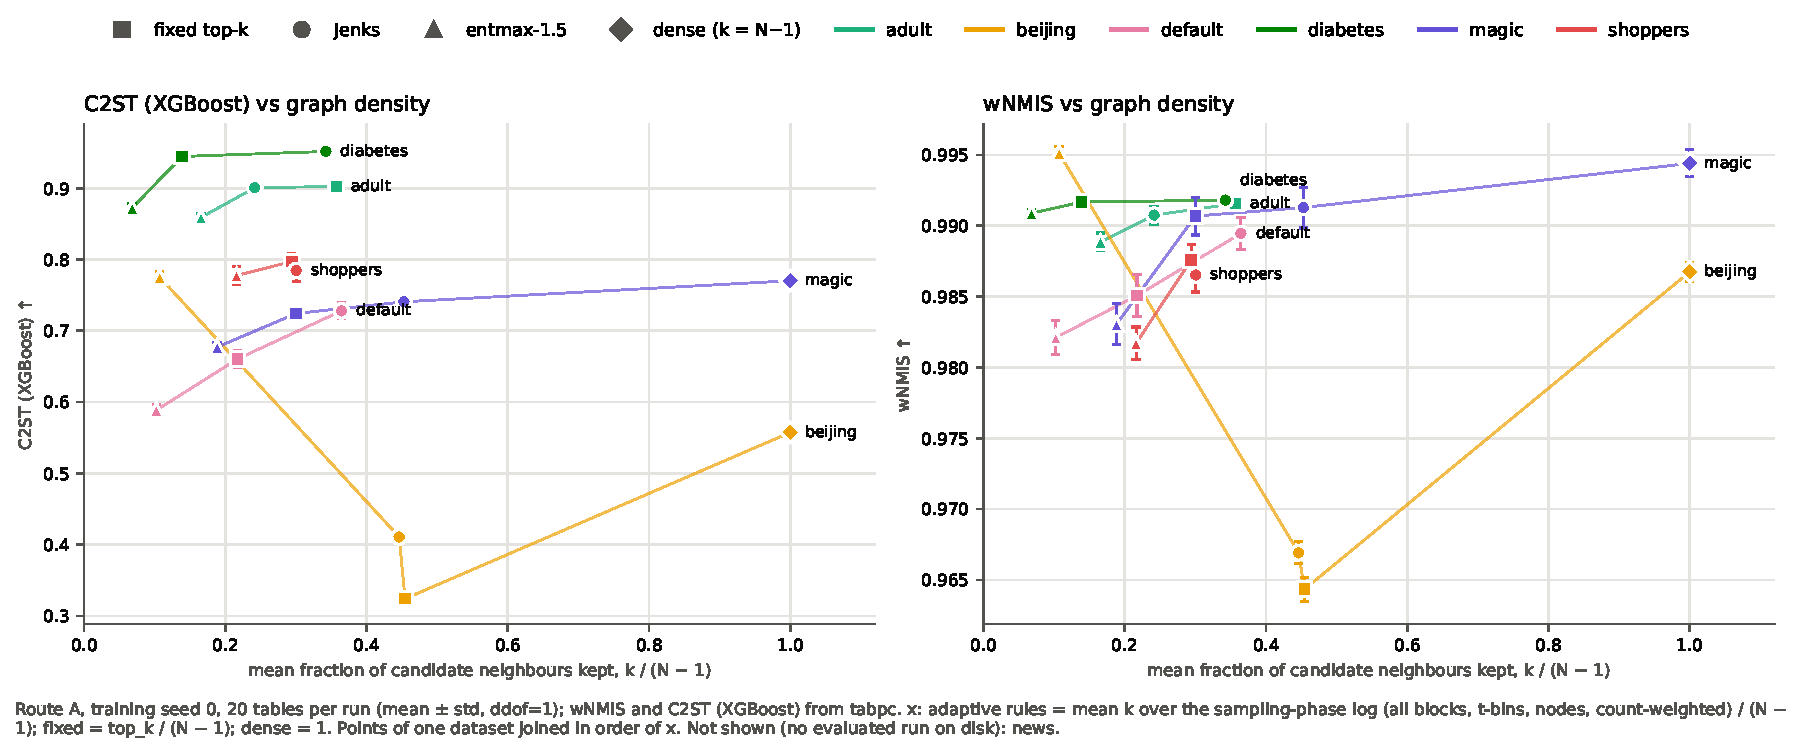
\includegraphics[width=\textwidth]{density_vs_fidelity.pdf}
  \caption[density vs fidelity]{Joint-distribution fidelity against the density of the learned graph. The horizontal axis is the mean percentage of the $N-1$ candidate neighbours that a node keeps during sampling: for the adaptive rules the count-weighted mean of the logged $k$ over all blocks, diffusion times and nodes, divided by $N-1$; for the fixed rule $k/(N-1)$; for the dense ablation 100\%. (a) C2ST with an XGBoost discriminator and (b) wNMIS (both from tabpc; higher is better), mean $\pm$ std over the 20 tables. Colour = dataset (lines join the runs of one dataset in order of density), marker = rule. Route A, training seed 0, 20 sampled tables. The adaptive rules' logged $k$ counts edges with a non-zero weight, so a kept edge whose weight underflows to zero counts as dropped (at most $2.6\times 10^{-4}$ of node evaluations). News not shown (no evaluated run yet).
}
  \label{fig:density_vs_fidelity}
\end{figure}

\begin{figure}[p]
  \centering
  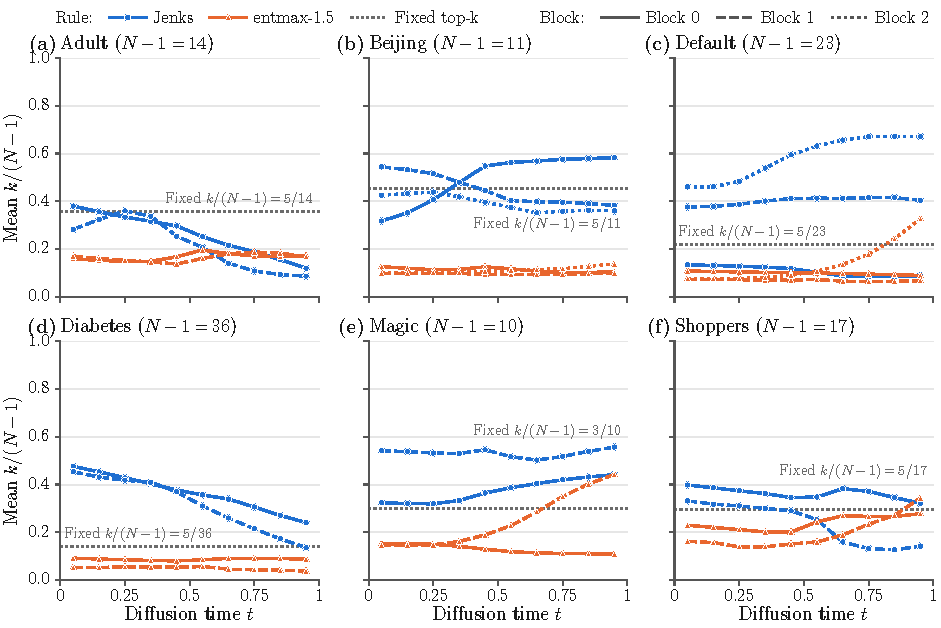
\includegraphics[width=\textwidth]{topk_frac_vs_t.pdf}
  \caption[topk frac vs t]{Mean fraction of the $N-1$ candidate neighbours that a node keeps, $k/(N-1)$, during sampling, as a function of the diffusion time $t$ ($t=0$: clean data, $t=1$: pure noise), for the two adaptive rules (colour) in each GNN block (line style). Each point averages the selected $k$ over all nodes and all denoiser calls whose $t$ falls in a bin of width 0.1 (weighted by count), over the 20 sampled tables. The dotted grey line is the fixed top-$k$ rule's constant $k/(N-1)$; $N-1$ is the number of other columns. Route A, training seed 0, 20 sampled tables. Runs with $k$ statistics: Jenks: Adult, Beijing, Default, Diabetes, Magic, Shoppers; entmax-1.5: Adult, Beijing, Default, Diabetes, Magic, Shoppers. No adaptive-rule run of News has $k$ statistics yet.
}
  \label{fig:topk_frac_vs_t}
\end{figure}

\begin{figure}[p]
  \centering
  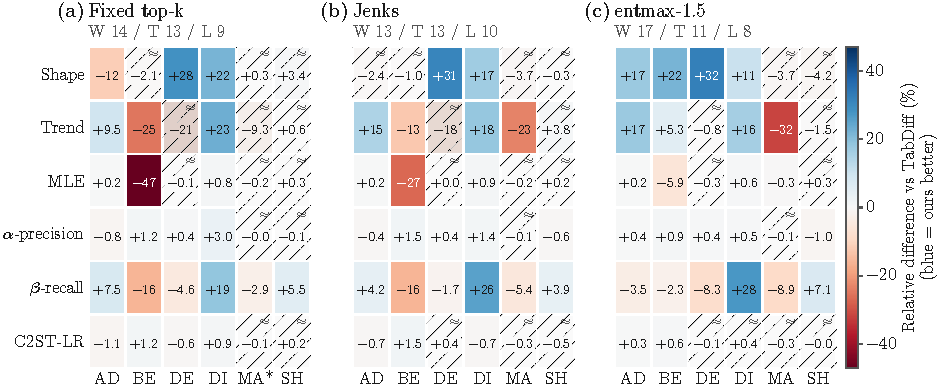
\includegraphics[width=\textwidth]{vs_tabdiff_reldiff.pdf}
  \caption[vs tabdiff reldiff]{Relative difference between our AttnGNN denoiser inside TabDiff and TabDiff as reported in its paper, for (a) the fixed top-$k$ rule, (b) Jenks and (c) entmax-1.5, on the six metrics the TabDiff paper reports (MLE: AUC, or RMSE on Beijing). Each cell is the signed difference in percent of TabDiff's value, oriented so that positive (blue) means ours is better: $(\text{TabDiff} - \text{ours})/\text{TabDiff}$ for Shape and Trend errors and RMSE, $(\text{ours} - \text{TabDiff})/\text{TabDiff}$ for AUC, $\alpha$-precision, $\beta$-recall and C2ST-LR. Values are rounded to one decimal below 10\% and to integers above. Hatched, paler cells marked $\approx$ in the corner are ties: the difference is within our standard deviation over the 20 tables (the rule of the win/tie/loss table); the panel subtitles count wins / ties / losses. Shared colour scale $\pm47$\% (largest magnitude 46.7\%). In panel (a) the Magic column (MA*) is the dense run ($k = N-1 = 10$), as in the result tables; with the sparse fixed run ($k=3$) its Trend, MLE and $\alpha$-precision cells would be losses instead of ties. Datasets: AD = Adult, BE = Beijing, DE = Default, DI = Diabetes, MA = Magic, SH = Shoppers. Route A, training seed 0, 20 sampled tables; News is not shown (no evaluated run yet).
}
  \label{fig:vs_tabdiff_reldiff}
\end{figure}

\begin{figure}[p]
  \centering
  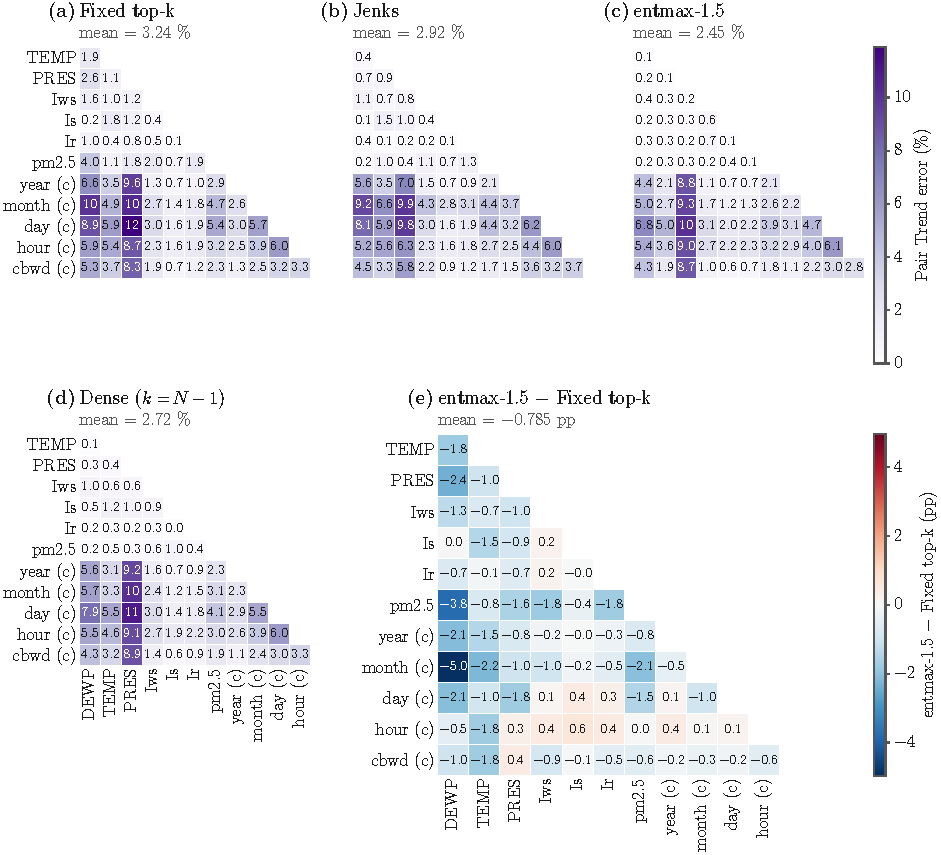
\includegraphics[width=\textwidth]{pair_trend_error_beijing.pdf}
  \caption[pair trend error beijing]{Pair-wise Trend error on Beijing: for every pair of columns, $100\,(1-\text{score})$ of the Column Pair Trends metric that TabDiff's evaluation computes (correlation similarity for two numerical columns, contingency similarity otherwise), averaged over the 20 sampled tables; lower is better. Panels: (a) Fixed top-k, (b) Jenks, (c) entmax-1.5, (d) Dense ($k = N-1$), and (e) the difference entmax-1.5 $-$ Fixed top-k in percentage points (blue: the adaptive rule is better). Each panel's subtitle gives the mean over all pairs, which equals the run's Trend error. Columns are in TabDiff's evaluation order, numerical first, categorical columns marked (c). Values $\geq 10$ are rounded to integers. Route A, training seed 0, 20 sampled tables.
}
  \label{fig:pair_trend_error_beijing}
\end{figure}

\begin{figure}[p]
  \centering
  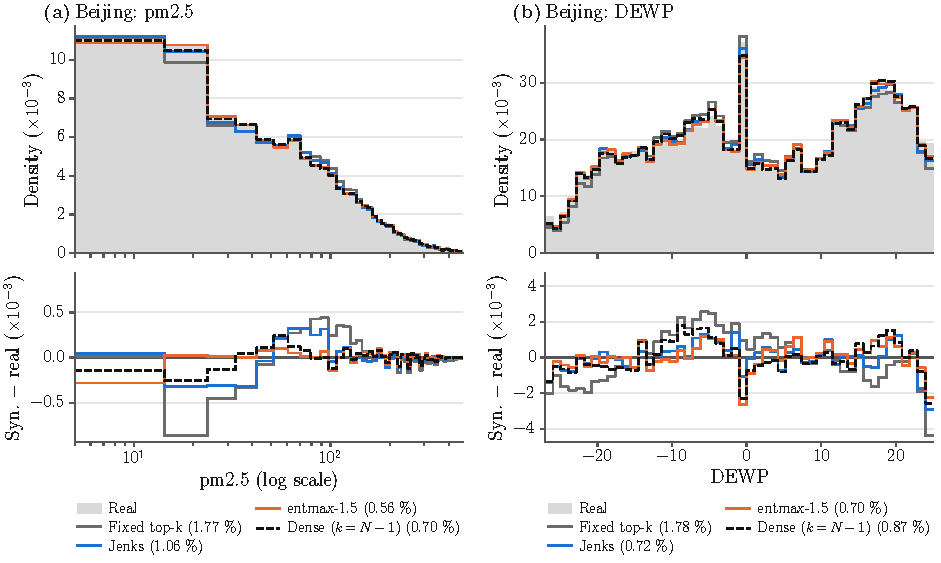
\includegraphics[width=\textwidth]{marginals.pdf}
  \caption[marginals]{Marginal distributions of two numerical columns of Beijing (pm2.5, DEWP) under each rule. Top: density of the real training data (grey) and of the synthetic data, pooled over the 20 sampled tables (lines); bottom: synthetic minus real density per bin, where the differences behind the Shape error become visible. Bins: 50 equal-width bins between the real 0.5\% and 99.5\% quantiles; both densities are counts divided by (all rows $\times$ bin width), so mass outside the window lowers the curve instead of being renormalised. The percentage after each rule in the legend is that rule's Shape error of the column ($100\,(1-\text{KS complement})$, mean over the 20 tables). The x axis of pm2.5 is logarithmic (heavy right tail). Route A, training seed 0, 20 sampled tables.
}
  \label{fig:marginals}
\end{figure}

\begin{figure}[p]
  \centering
  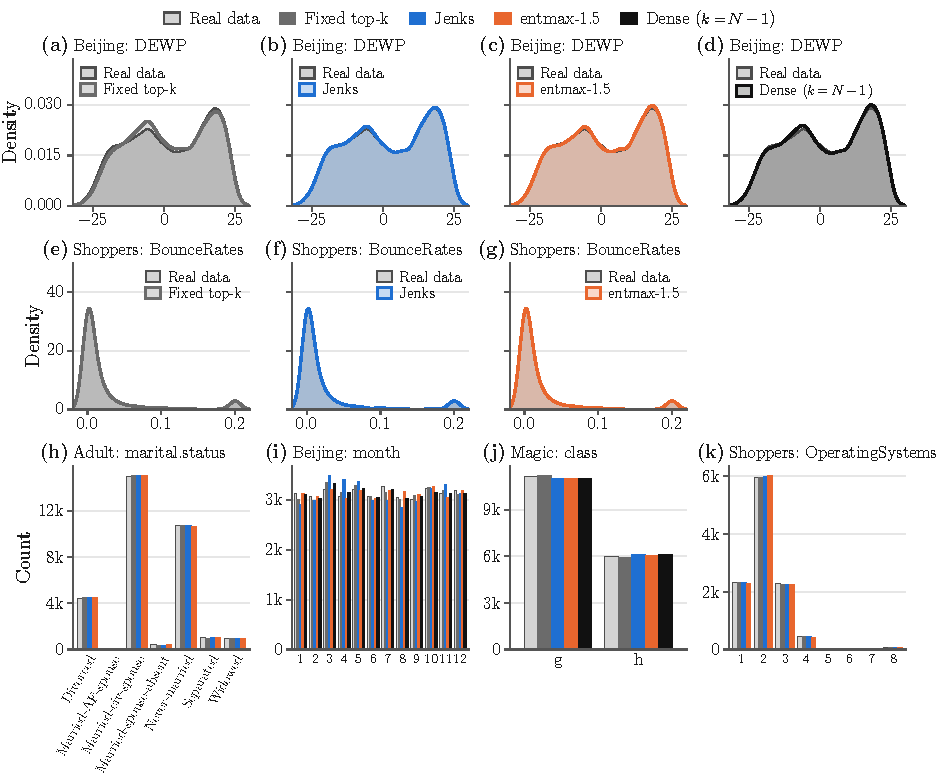
\includegraphics[width=\textwidth]{paper_style_marginals.pdf}
  \caption[paper style marginals]{Marginal distributions of the columns shown in Figure~3 of the TabDiff paper, for each of our neighbour-selection rules (Fixed top-$k$, Jenks, entmax-1.5). (a)--(f): kernel density estimates of two numerical columns (Beijing DEWP, Shoppers BounceRates), real data in grey and each rule's synthetic data in its colour; real and synthetic densities in a panel use the same bandwidth (Scott's rule on the real data), and the synthetic estimate pools the 20 sampled tables (subsampled to 200{,}000 rows with a fixed seed); the axis spans the real 0.5--99.5\% quantiles extended by 10\%, and the panels of a row share their $y$-axis. (g)--(j): category counts of four categorical columns ({bd}), real table (grey) and each rule's mean over the 20 tables (synthetic tables have the real table's size). Layout and columns follow the TabDiff paper so that the rules can be set beside its Figure~3, but the paper's panels show other models on other samples: the comparison is visual and qualitative only. Fixed top-$k$ on Magic is the $k=3$ run. Real data: the training table TabDiff's evaluation compares against. Route A, training seed 0, 20 sampled tables.
}
  \label{fig:paper_style_marginals}
\end{figure}

\begin{figure}[p]
  \centering
  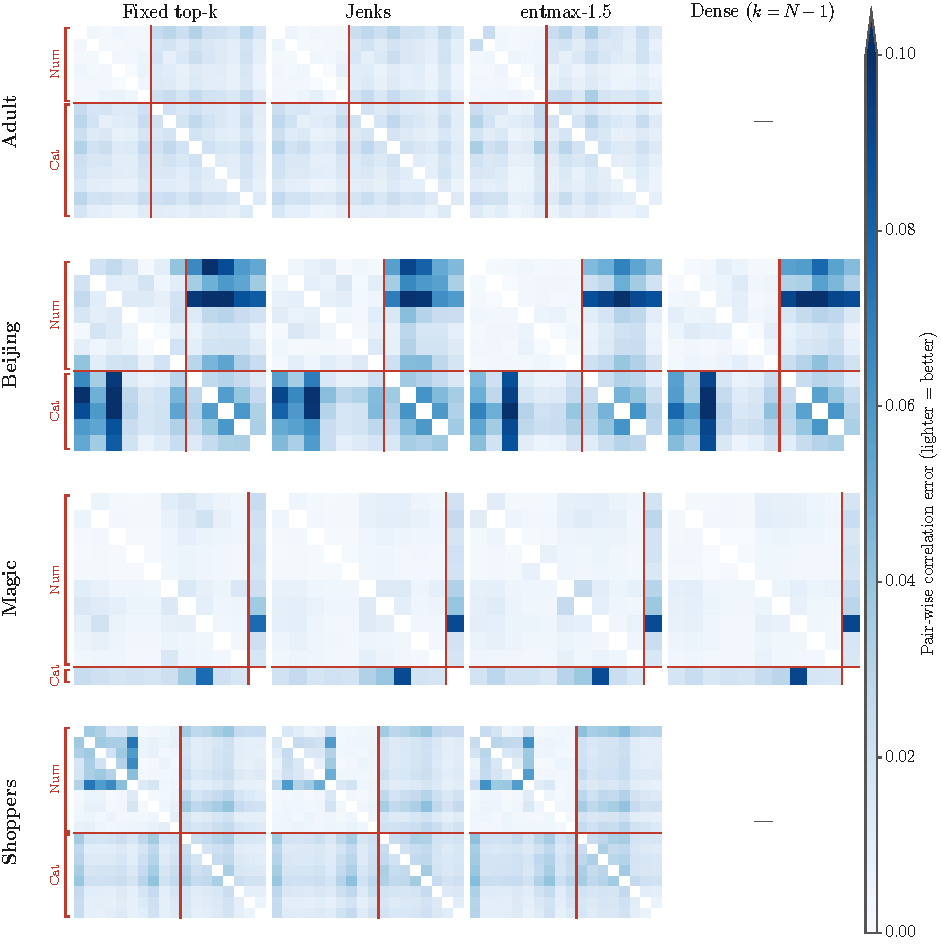
\includegraphics[width=\textwidth]{paper_style_pair_heatmaps.pdf}
  \caption[paper style pair heatmaps]{Pair-wise correlation error of every pair of columns, with the colour scale of Figure~4 of the TabDiff paper, for our three neighbour-selection rules (Fixed top-$k$, Jenks, entmax-1.5) on Adult, Beijing, Default, Diabetes, Magic and Shoppers. Each cell of a matrix is $1-\text{score}$ of the Column Pair Trends metric of sdmetrics~0.18.0 as computed inside TabDiff's evaluation (correlation similarity for two numerical columns, contingency similarity otherwise), averaged over the 20 sampled tables; the matrix is symmetric, its diagonal is left white, and the columns are ordered numerical first, then categorical (red lines and brackets). Colour scale 0 to 0.10 as in the paper (lighter is better); values above 0.10 are drawn at the maximum colour. Per dataset, the mean of each matrix, which equals the run's Trend error divided by 100, and in brackets the percentage of pairs above 0.10 (Fixed top-$k$ / Jenks / entmax-1.5): Adult: 0.013 / 0.013 / 0.012 (0.0\% / 0.0\% / 0.0\%); Beijing: 0.032 / 0.029 / 0.025 (3.0\% / 0.0\% / 1.5\%); Default: 0.031 / 0.030 / 0.026 (7.2\% / 14.5\% / 3.6\%); Diabetes: 0.017 / 0.018 / 0.019 (0.5\% / 0.5\% / 0.8\%); Magic: 0.010 / 0.009 / 0.010 (0.0\% / 0.0\% / 0.0\%); Shoppers: 0.017 / 0.017 / 0.018 (0.0\% / 0.0\% / 0.0\%). Fixed top-$k$ on Magic is the $k=3$ run; Magic's only categorical column is its target, a block too narrow for a label. The layout follows the TabDiff paper so that the rules can be set beside its Figure~4, but the paper's panels show other models on other samples: the comparison is visual and qualitative only; Default and Diabetes are not in the paper's Figure~4, so for them there is no counterpart to compare with. Route A, training seed 0, 20 sampled tables.
}
  \label{fig:paper_style_pair_heatmaps}
\end{figure}

\begin{figure}[p]
  \centering
  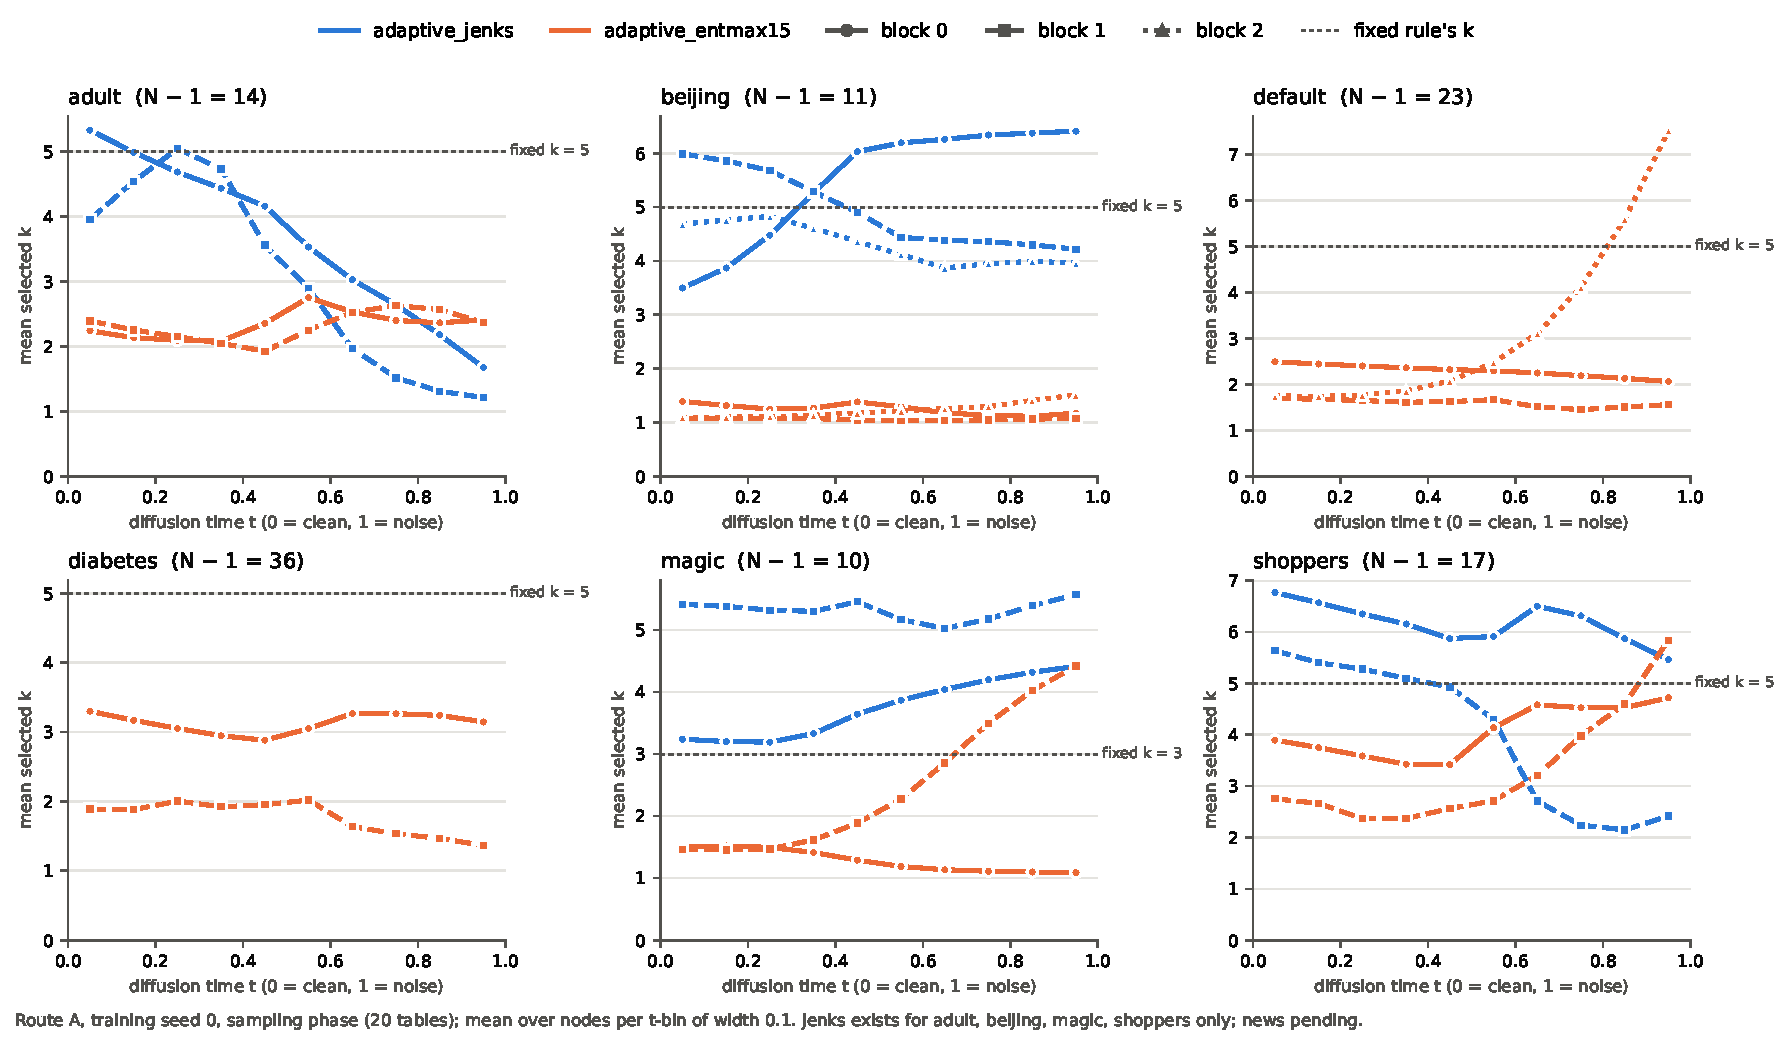
\includegraphics[width=\textwidth]{topk_k_vs_t.pdf}
  \caption[topk k vs t]{Mean number of neighbours $k$ that a node keeps, during sampling, as a function of the diffusion time $t$ ($t=0$: clean data, $t=1$: pure noise), for the two adaptive rules (colour) in each GNN block (line style). Each point averages the selected $k$ over all nodes and all denoiser calls whose $t$ falls in a bin of width 0.1 (weighted by count), over the 20 sampled tables. The dotted grey line is the fixed top-$k$ rule's constant $k$; $N-1$ is the number of other columns. Route A, training seed 0, 20 sampled tables. Runs with $k$ statistics: Jenks: Adult, Beijing, Default, Diabetes, Magic, Shoppers; entmax-1.5: Adult, Beijing, Default, Diabetes, Magic, Shoppers. No adaptive-rule run of News has $k$ statistics yet.
}
  \label{fig:topk_k_vs_t}
\end{figure}

\begin{figure}[p]
  \centering
  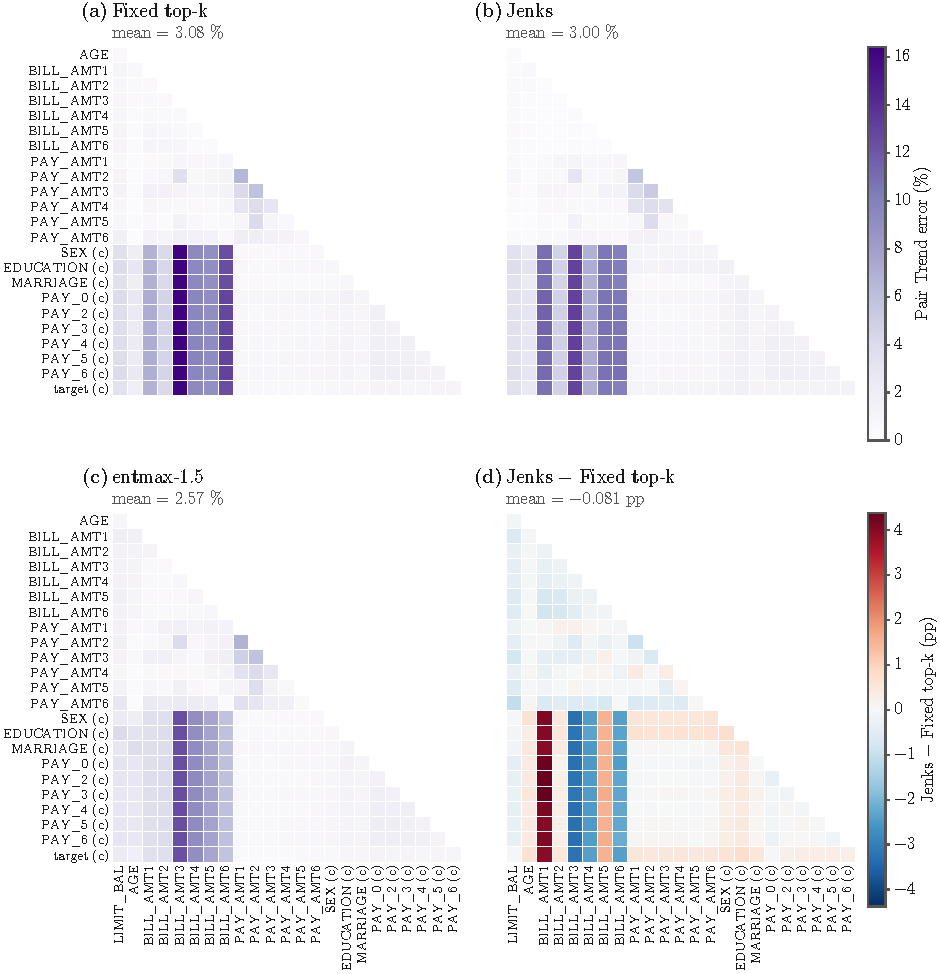
\includegraphics[width=\textwidth]{pair_trend_error_default.pdf}
  \caption[pair trend error default]{Pair-wise Trend error on Default: for every pair of columns, $100\,(1-\text{score})$ of the Column Pair Trends metric that TabDiff's evaluation computes (correlation similarity for two numerical columns, contingency similarity otherwise), averaged over the 20 sampled tables; lower is better. Panels: (a) Fixed top-k, (b) Jenks, (c) entmax-1.5, and (d) the difference Jenks $-$ Fixed top-k in percentage points (blue: the adaptive rule is better). Each panel's subtitle gives the mean over all pairs, which equals the run's Trend error. Columns are in TabDiff's evaluation order, numerical first, categorical columns marked (c); ``target'' = default payment next month. Route A, training seed 0, 20 sampled tables.
}
  \label{fig:pair_trend_error_default}
\end{figure}

\begin{figure}[p]
  \centering
  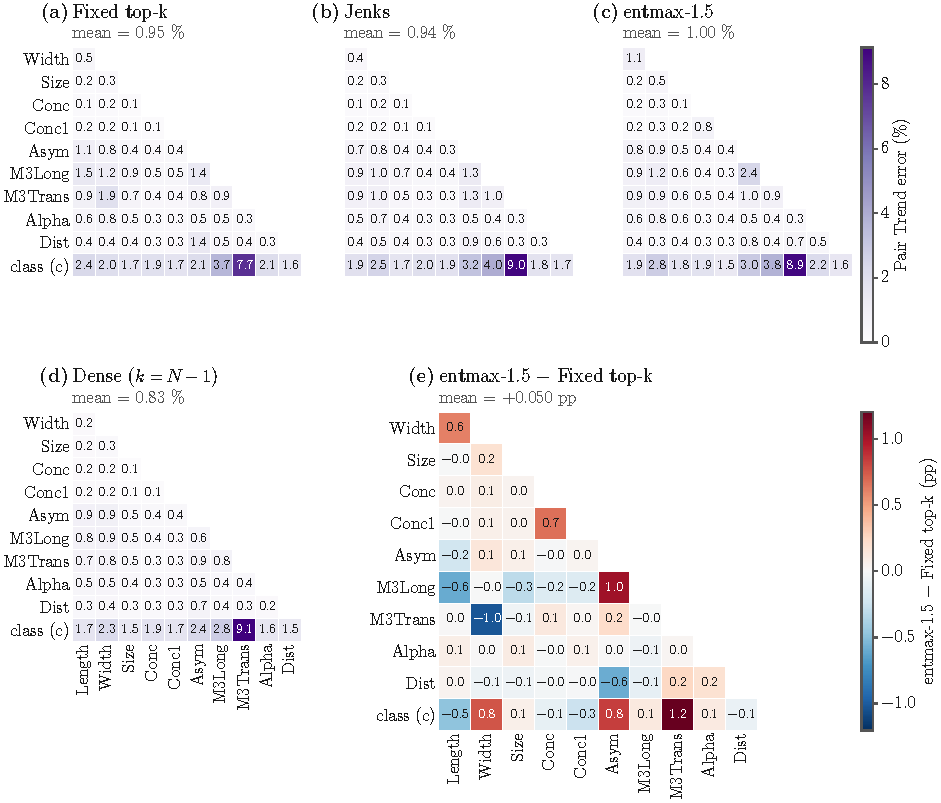
\includegraphics[width=\textwidth]{pair_trend_error_magic.pdf}
  \caption[pair trend error magic]{Pair-wise Trend error on Magic: for every pair of columns, $100\,(1-\text{score})$ of the Column Pair Trends metric that TabDiff's evaluation computes (correlation similarity for two numerical columns, contingency similarity otherwise), averaged over the 20 sampled tables; lower is better. Panels: (a) Fixed top-k, (b) Jenks, (c) entmax-1.5, (d) Dense ($k = N-1$), and (e) the difference entmax-1.5 $-$ Fixed top-k in percentage points (blue: the adaptive rule is better). Each panel's subtitle gives the mean over all pairs, which equals the run's Trend error. Columns are in TabDiff's evaluation order, numerical first, categorical columns marked (c). Values $\geq 10$ are rounded to integers. Route A, training seed 0, 20 sampled tables.
}
  \label{fig:pair_trend_error_magic}
\end{figure}

\begin{figure}[p]
  \centering
  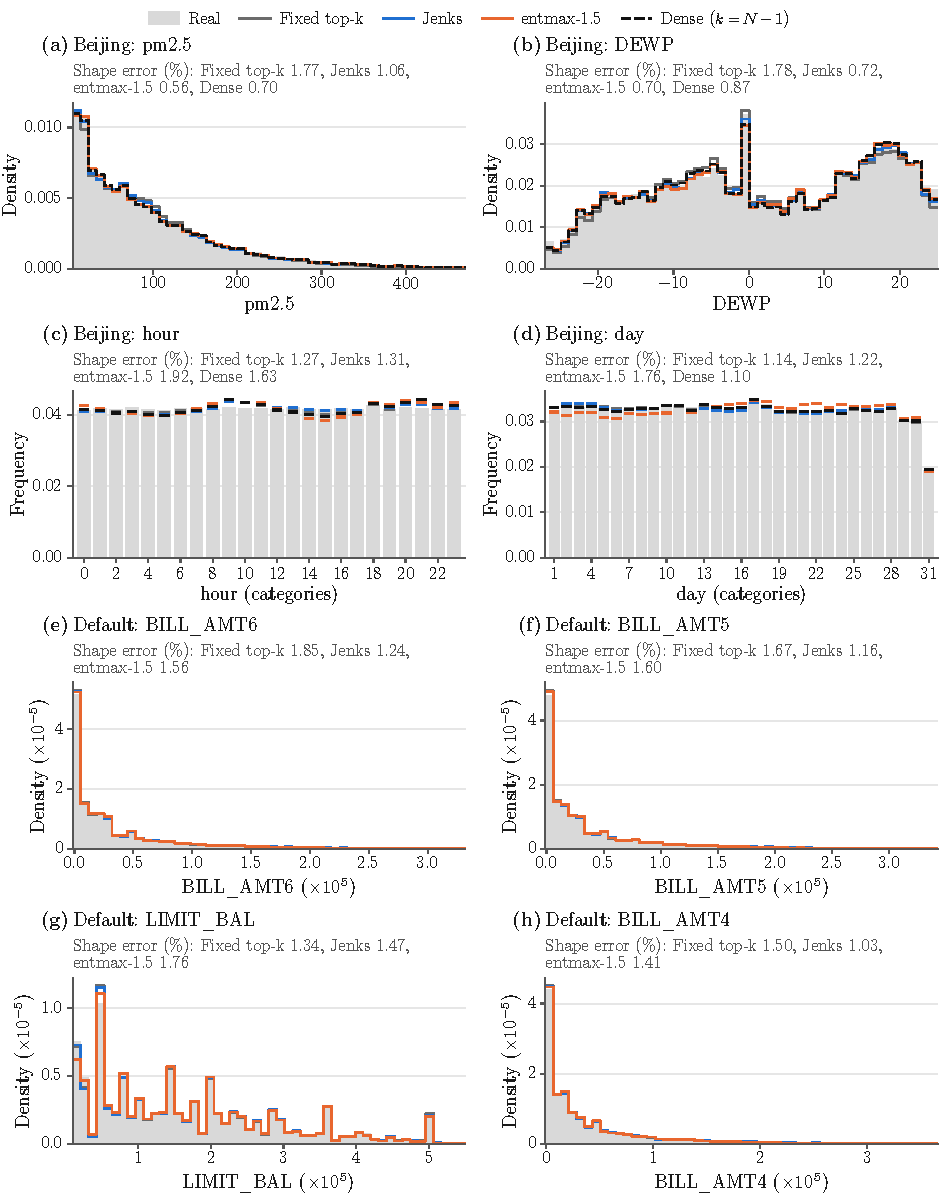
\includegraphics[width=\textwidth]{marginals_appendix.pdf}
  \caption[marginals appendix]{Marginals of automatically chosen columns (Beijing: pm2.5, DEWP, hour, day; Default: BILL\_AMT6, BILL\_AMT5, LIMIT\_BAL, BILL\_AMT4). Per dataset: the two numerical columns whose Shape error differs most between the adaptive rule and the fixed rule (entmax-1.5 on Beijing, Jenks on Default), then the two other columns with the largest Shape error under the best rule (lowest mean Shape error: Beijing entmax-1.5, Default entmax-1.5). Numerical columns: real density (grey) and each rule's synthetic density pooled over the 20 tables, 50 bins between the real 0.5\% and 99.5\% quantiles, counts divided by (all rows $\times$ bin width). Categorical columns: real frequency (grey bars) and each rule's mean frequency over the 20 tables (ticks). Subtitles: Shape error of the column per rule. Route A, training seed 0, 20 sampled tables.
}
  \label{fig:marginals_appendix}
\end{figure}

\end{document}
